\chapter{ผลการทดลอง}
\label{chapter:result}

ในงานวิจัยนี้การทดลองถูกแบ่งออกเป็น 2 ส่วนหลัก ๆ คือ การจัดกลุ่มข้อมูลสองกลุ่ม (Binary Classification) และ การจัดกลุ่มข้อมูลหลายกลุ่ม (Multi-Class Classification) โดยประเภทของข้อมูลที่ถูกใช้ในการทดลองมี 2 ประเภท คือ ข้อมูลแบบมีโครงสร้าง และ ข้อมูลภาพ สำหรับข้อมูลแบบมีโครงสร้างจะมีทั้งหมด 23 ชุดข้อมูล ที่ซึ่งแต่ละชุดข้อมูลจะมีกลุ่มของข้อมูลอยู่ 2 กลุ่ม โดยชุดข้อมูลทั้งหมดนี้จะเป็นชุดข้อมูลที่ไม่สมดุลสำหรับการวัดเปรียบเทียบสมรรถนะเกณฑ์มาตรฐาน (Benchmark) ตามที่ถูกนำเสนอไปใน~\cite{Ding:2011} สำหรับข้อมูลภาพจะมี 2 ชุดข้อมูล คือ CIFAR-100~\cite{Krizhevsky:2009} และ CIFAR-10~\cite{Krizhevsky:2009} โดยทั้งสองนี้เป็นชุดข้อมูลที่สมดุลกันอยู่แล้ว และมีจำนวนกลุ่มข้อมูล 100 และ 10 กลุ่มตามลำดับ แต่จะถูกนำมาดัดแปลงให้ไม่สมดุลเพื่อทำการทดลอง โดยรายละเอียดของการดัดแปลงของ CIFAR-100 และ CIFAR-10 จะถูกอธิบายไว้ในหัวข้อย่อยต่อไป

สำหรับสถาปัตยกรรมของโมเดลที่ใช้ในการทดลองถูกแบ่งออกเป็น 2 ส่วน คือ โมเดลโครงข่ายประสาทเทียมแบบมี 1 Hidden Layer สำหรับการทดลองกับข้อมูลแบบมีโครงสร้าง และ โมเดล ResNet~\citep{He:2016} สำหรับการทดลองกับข้อมูลภาพ

\section{Binary Classification}
\subsubsection{ผลการทดลองกับชุดข้อมูลแบบมีโครงสร้าง}
\subsubsection{ผลการทดลองกับชุดข้อมูล CIFAR-100}
การทดลองใน~\cite{Wang:2016} ได้ทำการดัดแปลง CIFAR-100 โดยการแบ่งชุดข้อมูลออกเป็น 3 ชุดข้อมูลย่อย คือ Tree1, Tree2 และ Household และเลือกข้อมูลมา 2 กลุ่มที่แตกต่างกันสำหรับแต่ละชุดข้อมูลย่อย ที่ซึ่งข้อมูลในแต่ละชุดข้อมูลย่อยจะถูกทำให้ไม่สมดุลกัน สำหรับรายละเอียดของกลุ่มข้อมูลในแต่ละชุดข้อมูลย่อยดังนี้

\paragraph{Tree1}
เป็นชุดข้อมูลที่ประกอบด้วยข้อมูลของกลุ่ม \emph{maple tree} และ \emph{oak tree} โดยจะให้กลุ่ม \emph{maple tree} เป็นกลุ่มข้อมูลส่วนมาก และ \emph{oak tree} เป็นกลุ่มข้อมูลส่วนน้อย

\paragraph{Tree2}
เป็นชุดข้อมูลที่ประกอบด้วยข้อมูลของกลุ่ม \emph{maple tree} และ \emph{palm tree} โดยจะให้กลุ่ม \emph{maple tree} เป็นกลุ่มข้อมูลส่วนมาก และ \emph{palm tree} เป็นกลุ่มข้อมูลส่วนน้อย

\paragraph{Household}
เป็นชุดข้อมูลที่ประกอบด้วยข้อมูลของกลุ่ม \emph{household furniture} และ \emph{household electrical devices} โดยจะให้กลุ่ม \emph{household furniture} เป็นกลุ่มข้อมูลส่วนมาก และ \emph{household electrical devices} เป็นกลุ่มข้อมูลส่วนน้อย

รูปที่~\ref{fig:result-cifar100} แสดงผลการทดลองของแต่ละชุดข้อมูล โดยจากผลการทดลองสามารถสรุปได้ว่าฟังก์ชันสูญเสียแบบ Hybrid มีประสิทธิภาพเหนือกว่าฟังก์ชันสูญเสียอื่น ๆ อย่างสิ้นเชิง

\begin{figure}[h]
  \centering
  \subfigure[]{
      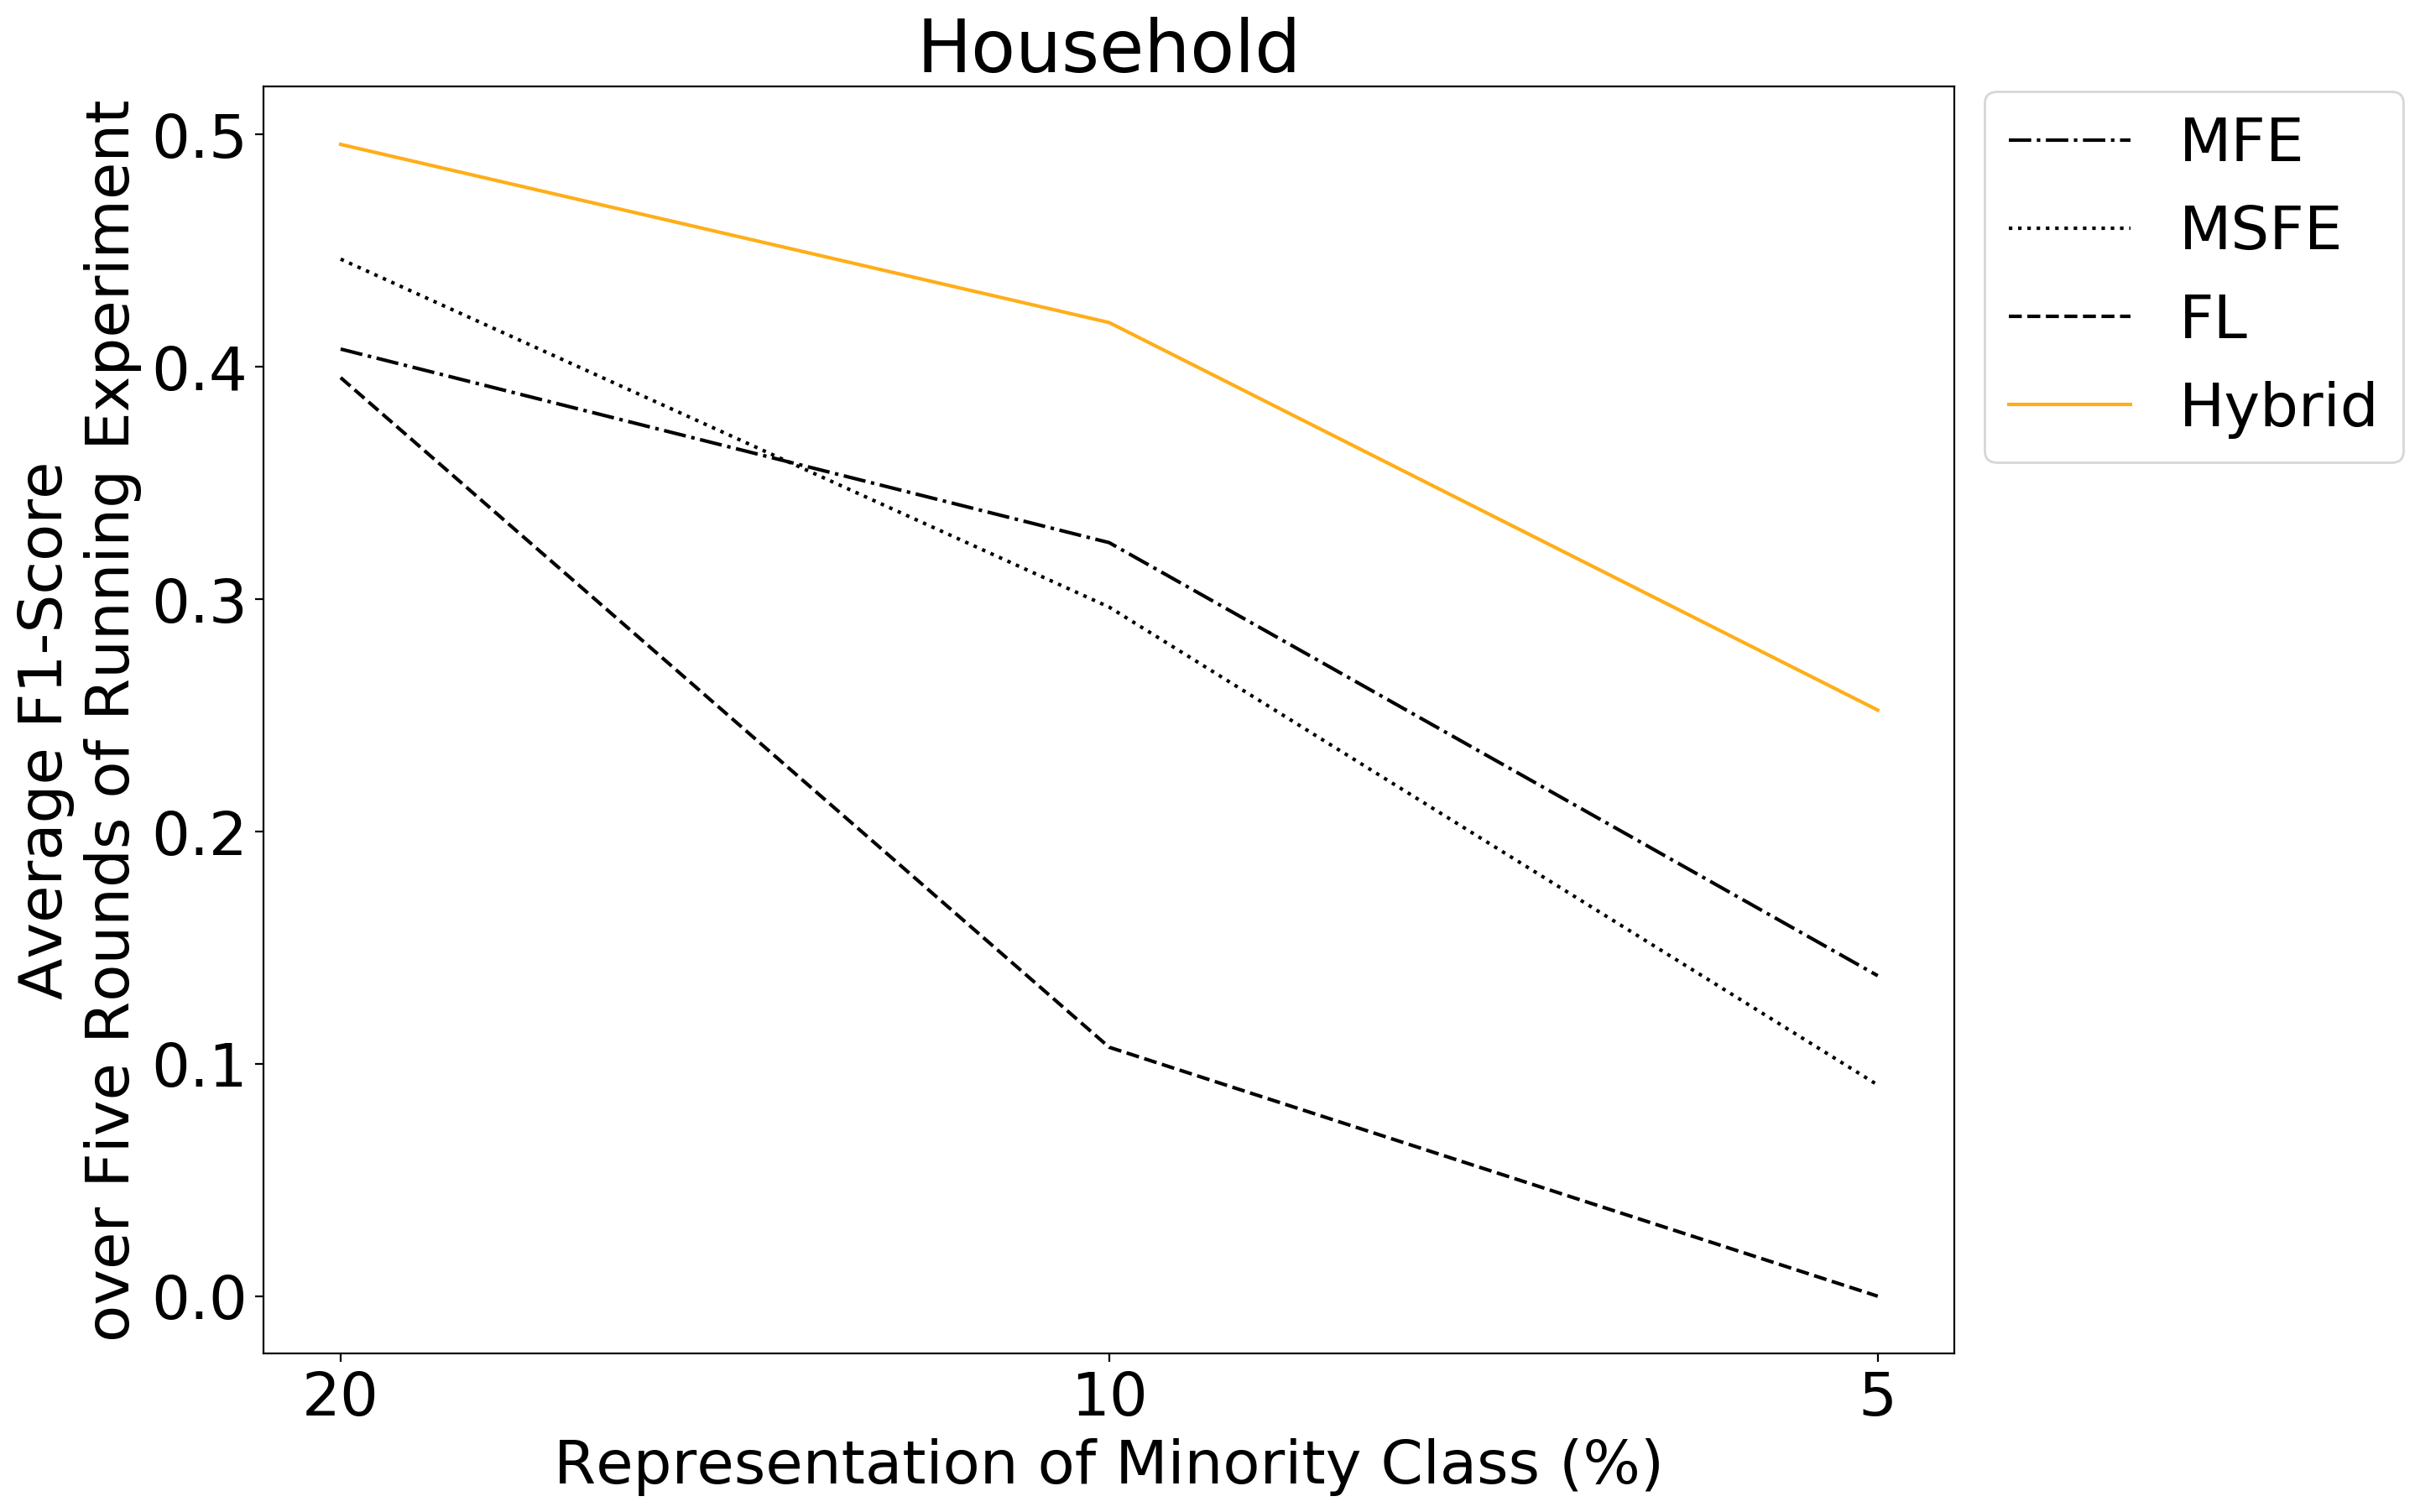
\includegraphics[width=0.45\columnwidth]{results/Household_cifar100.png}
      \label{fig:result-cifar100-household}
  }
  \subfigure[]{
      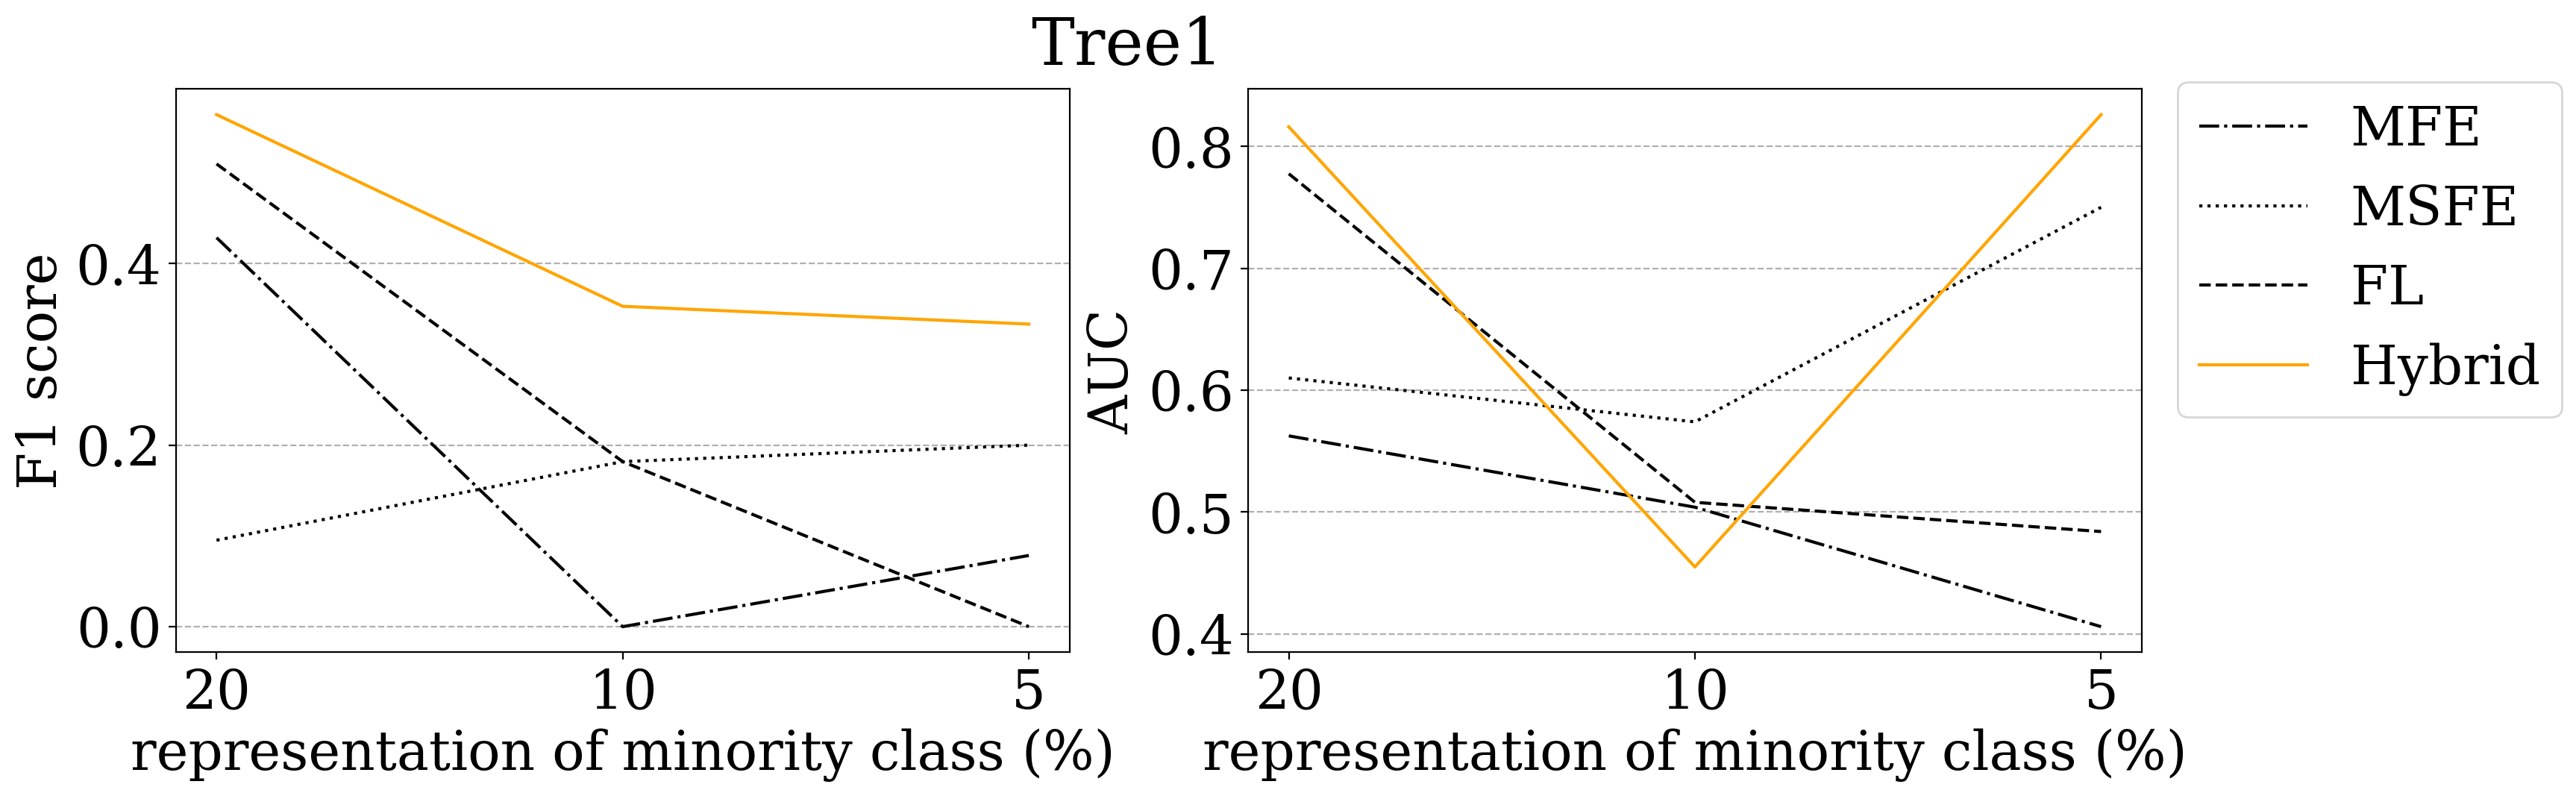
\includegraphics[width=0.45\columnwidth]{results/Tree1_cifar100.png}
      \label{fig:result-cifar100-tree1}
  }
  \subfigure[]{
    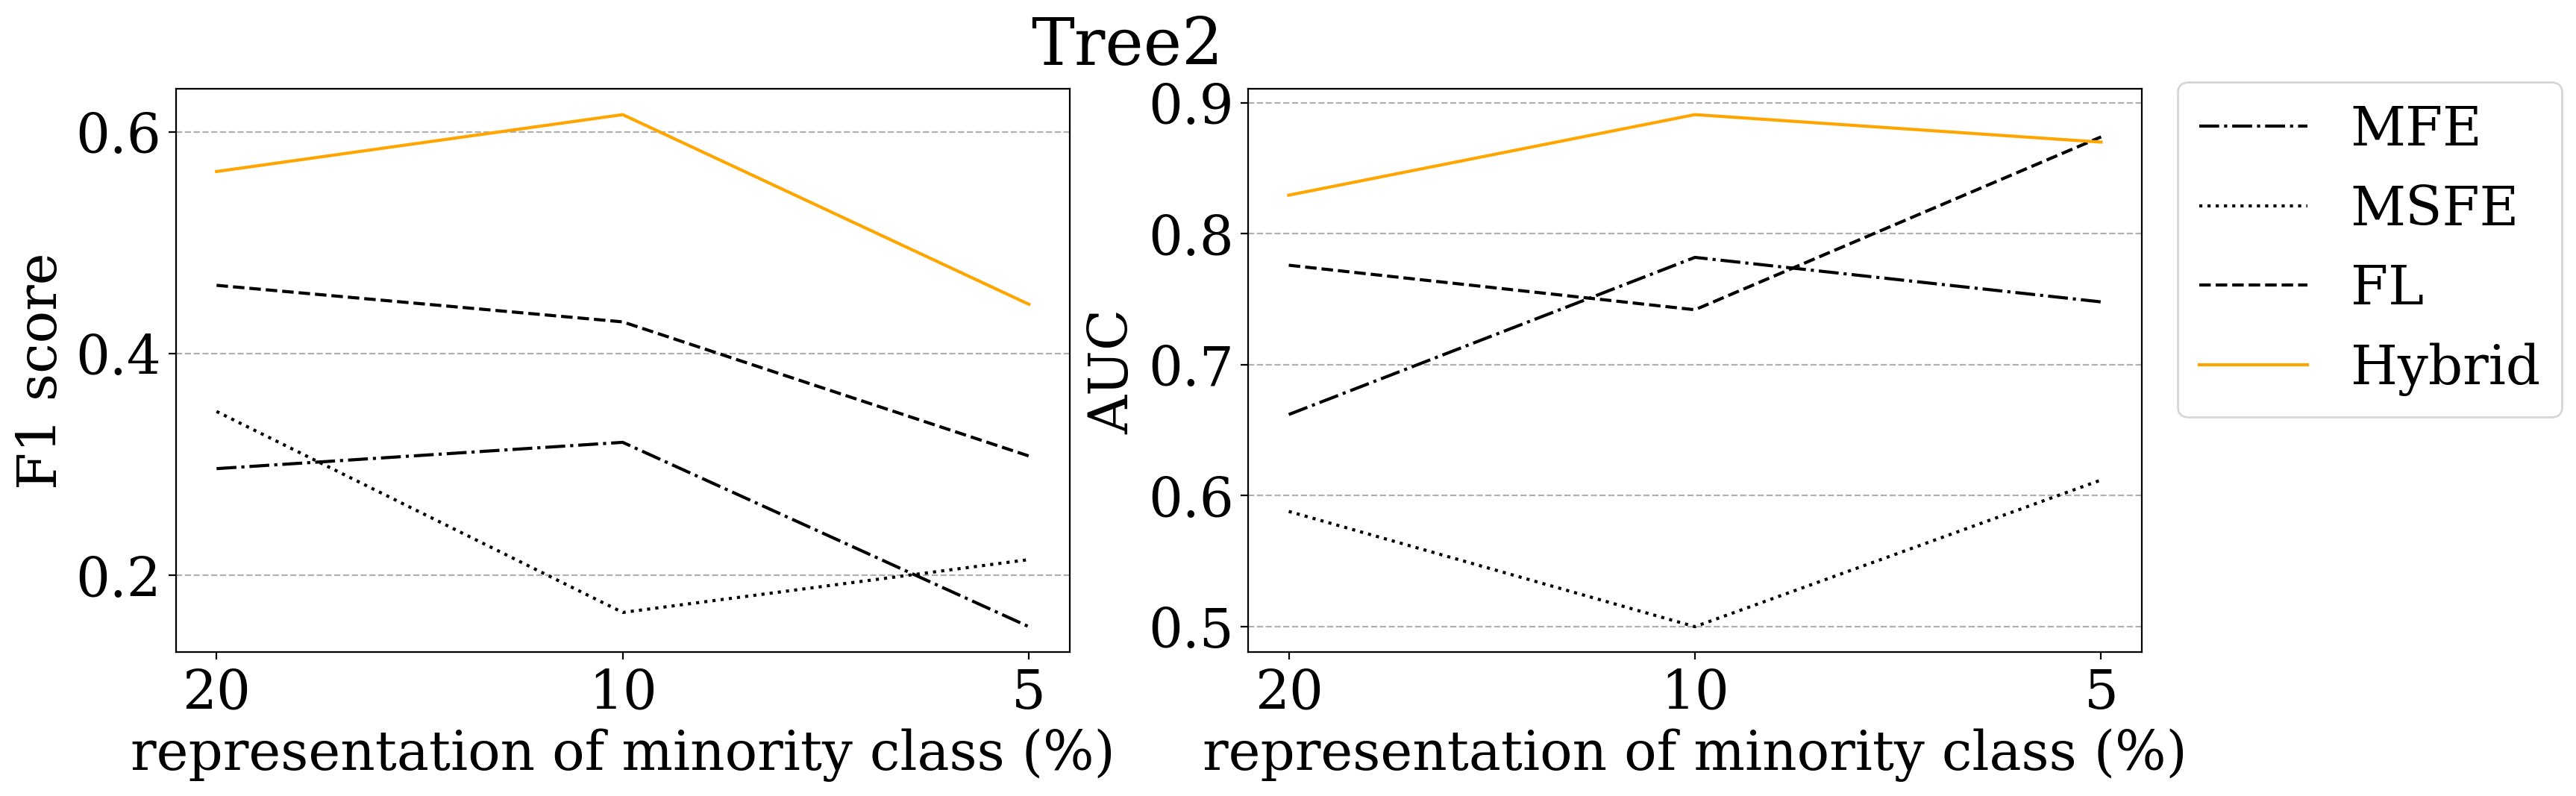
\includegraphics[width=0.45\columnwidth]{results/Tree2_cifar100.png}
    \label{fig:result-cifar100-tree2}
  }
  \caption{ประสิทธิภาพของแต่ละฟังก์ชันสูญเสีย เมื่อทดสอบกับชุดข้อมูลที่มีอัตราจำนวนตัวอย่างของกลุ่มข้อมูลส่วนน้อยที่แตกต่างกัน}
  \label{fig:result-cifar100}
\end{figure}
\FloatBarrier

\label{ex:cifar-100}
\section{Multi-Class Classification}
\subsubsection{ผลการทดลองกับชุดข้อมูล Long-Tailed-Imbalanced CIFAR-10}
ชุดข้อมูล CIFAR-10 จะถูกดัดแปลงให้ไม่สมดุลแบบ Long-Tail
\label{ex:long-tailed-cifar-10}
\subsubsection{ผลการทดลองกับชุดข้อมูล Step-Imbalanced CIFAR-10}
ชุดข้อมูล CIFAR-10 จะถูกดัดแปลงให้ไม่สมดุลแบบ Step
\label{ex:step-cifar-100}